\section{Linear Regression}

Linear Regression is a common and simple technique in the world of predictive analytics. One common example of linear regression is the fitting of straight lines to a graph. Linear Regression is considered a supervised machine learning technique. The data is usually not perfect, there is often a source of noise, this could be network latency.

\begin{equation}
    f(x) = mx+c
\end{equation}
This describes a straight line relationship, where y is the y-axis variable and x is the x-axis variable, the relationship between them is defined as m where m is the slope of the line. c is a constant or intercept where the line meets the y-axis

Linear regression will generally be used for fitting multiple coefficients. Coefficients mean lots of different features. For example, if we want to predict the weather, then to make an accurate model we would probably need multiple features such as wind speed and atmospheric pressure.

\begin{equation}
\hat{y} = \frac{1}{n}\sum_{i=1}^n y_i
\end{equation}

Y hat is the predicted value of y. Beta 0 corresponds to to the intercept value. Sum of, is iterating over the features denoted by k. k can be described as the k co-efficient values for a feature.

\subsection{Linear Regression Features}

Linear regression works by finding a straight line relationship between a set of features (coefficients). Features could be anything from miles per gallon of a new car to the frequency of a CPU. One caveat with these features is that in linear regression they must be expressed numerically. For example, if we have a feature x which denotes the gender of a human as either 'M', 'F'. We could not input these values into our regression as they are not numeric. These values could not be used in our regression without being transformed. One of the methods of data transformation is called one hot encoding. 

\subsection{Feature Transformations}

There are certain cases where a feature transformation is required. As mentioned earlier we would need one hot encoding to make sure our data is numeric. Using our example of a gender feature above, one hot encoding will take the string values 'M' and 'F' and convert them to numbers. Interestingly it will not replace our gender column, instead, it will create 2 more features. We will end up with a new male and female feature encoded with a 1 for a true value and a 0 for a false value.
Transformations can be used to account for a non-linear relationship between our features and the predictor. Non-linear relationships can be difficult to find and usually relies on a deep understanding of the the data. Once we have this understanding we can start to ask questions such as can the slope of
the relationship between Xi and E(Y) be expected to have the same sign for all values of Xi. Should we expect the magnitude of the slope to increase as Xi increases, or should we expect
the magnitude of the slope to decrease as Xi increases?\cite{nonlinearRelationships}

\subsection{Residuals vs fits plot}

One way to detect non-linearity in a dataset is to use residuals vs fits plots. It is a scatter plot of residuals on the y-axis and fitted values (estimated responses) on the x-axis. The plot is used to detect non-linearity, unequal error variances, and outliers \cite{residualsVsFitsPlot}. this residual plot may be used to check for violations in model assumptions particularly related to incorrect specification or presence of heteroscedasticity\cite{doi:10.1002/9781118625590.ch2}. Let's look at a simple linear regression model

\[ Y = \beta_0 + \beta_1X + \epsilon \]

The error terms are assumed to be normally distributed, homoscedastic(every value has the same variance) and are independent of one another. If these assumptions are correct than the observed residuals should be approximately normally distributed with constant variants for all the X values.

\begin{figure}[H]
  \centering
  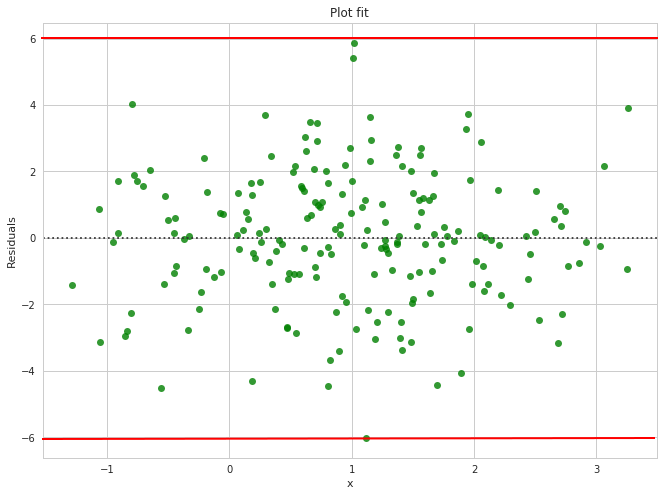
\includegraphics[scale=0.5,width=100mm]{./images/plotfit-good.png}
  \caption{Fit plot showing a good indication that the assumptions of our model are correct}
  \label{fig:fitsplotgood}
\end{figure}

In figure \ref{fig:fitsplotgood} we can see that variability is roughly the same for all the different values of X between the 2 red lines. There also does not appear to be much curvature or any other indications that there is a problem with our model. figure \ref{fig:fitsplotgood} gives us no indication that the assumptions of our model are false

\begin{figure}[H]
  \centering
  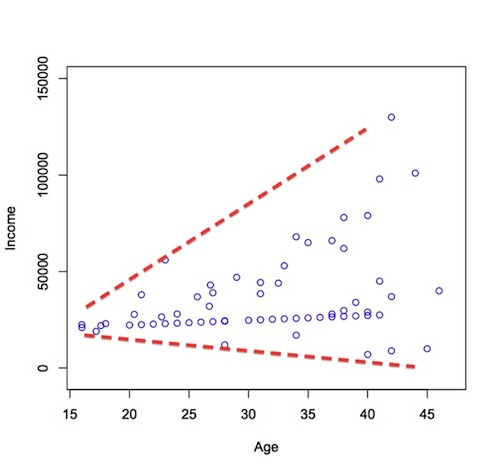
\includegraphics[scale=0.5,width=100mm]{./images/heteroscedasticity.jpg}
  \caption{Fit plot showing heteroscedasticity}
  \label{fig:fitsplotbad}
\end{figure}

In figure \ref{fig:fitsplotbad} \cite{heteroscedasticity} there are more obvious problems. The variants of the residuals increase with the x-axis. This would be considered a violation of our constant variable assumption. One option to deal with this situation is to use a technique called weighted regression. However overall our model assumptions are incorrect for this model.

\subsection{Measuring Model Errors}

If we are using linear regression to predict values, then we will need to measure the errors to prevent over-fitting or under-fitting.
\begin{figure}[H]
  \centering
  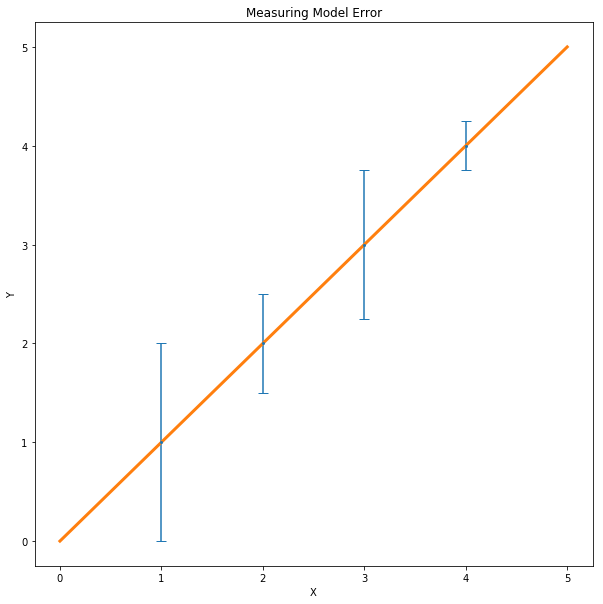
\includegraphics[scale=0.5,width=100mm]{./images/graph-error-bars.png}
  \caption{Linear regression with errors}
  \label{fig:graph-error-bars}
\end{figure}
In figure \ref{fig:graph-error-bars} we can see a linear model graph showing error levels. Each vertical bar represents some degree of an error. The further away from the straight orange line the greater the error. We can use the formula below to determine the error for each bar.
\begin{equation}
    \epsilon_i = y_i - \hat y_i
\end{equation}
Generally speaking, if the error is less than zero this means that we have overestimated the values. If the error is greater than zero than the prediction is less than the true value. If our error is zero then it can be considered accurate.

The equation mentioned above is good when dealing with single values. However, if we have a dataset with many features it may be more useful to measure the errors with a histogram.

\begin{figure}[H]
  \centering
  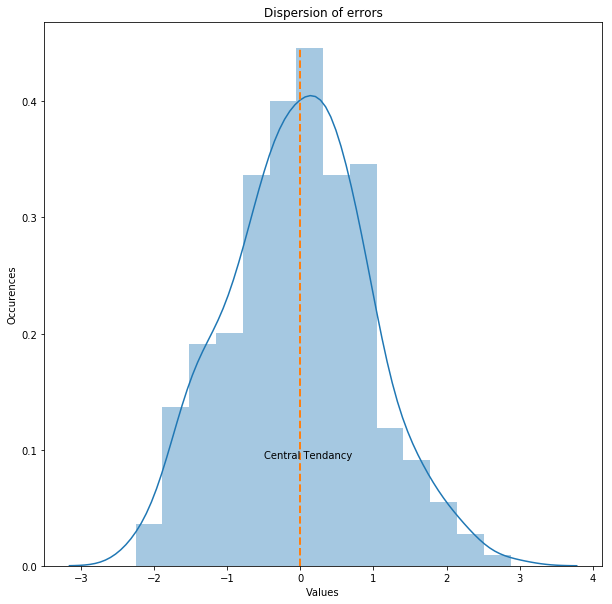
\includegraphics[scale=0.5,width=100mm]{./images/graph-histogram.png}
  \caption{Histogram showing central tendency and dispersion of errors}
  \label{fig:graph-histogram}
\end{figure}
Figure \ref{fig:graph-histogram} shows a histogram which could be used for multiple features. The dashed orange line is called the central tendency. We can see that this particular graph is showing that errors will occur between -2.2 and +2.9, this is known as the dispersion of errors.

\subsection{Least Squares}

Least squares is a widely used technique for finding the best fitting curve to a set of data points by minimizing the sum of the squares of the residuals. Least squares technique tend to penalize large residuals as the difference between the residual and the actual value is squared and then summed up with the rest of the differences.

\begin{equation}
RSS=\sum^n_{i=1}(\hat{y_i}- y_i)^2
\end{equation}
The error, epsilon, for a single value can be expressed as
\begin{equation}
\epsilon = (\hat{y_i}- y_i)^2
\end{equation}
\begin{equation}
RMSE = \sqrt\frac{\sum\limits_{i=1}^{n}(y_i-\hat{y_i})^2}{n}
\end{equation}
\begin{equation}
RSS = \sum^n_{i=1}\epsilon_i^2
\end{equation}
We can see that the definition of a root mean square error of the RMSE equation that RSS could be expressed in relation to RMSE
\begin{equation}
RSS = nRMSE^2
\end{equation}

\subsection{K Nearest Neighbours}

K nearest neighbours is a simple classification algorithm. Its purpose is to separate data points into classes so that new data points can easily be classified.
\begin{figure}[H]
  \centering
  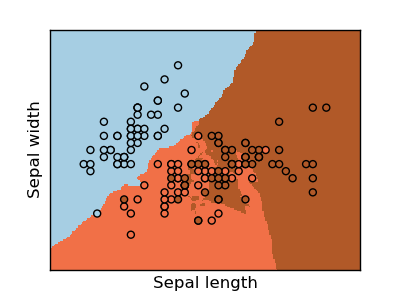
\includegraphics[scale=0.5,width=100mm]{./images/k-nearest-neighbours-example.png}
  \caption{Example of k nearest neighbours for the iris dataset}
  \label{fig:k-nearest-neighbours-example}
\end{figure}
Figure \ref{fig:k-nearest-neighbours-example} \cite{kNearestNeighboursExample}. Shows an example of k nearest neighbours classification in action for the iris dataset in sklearn. We can see that each of the data points lies in one of the classification zones. KNN is considered a lazy algorithm because it requires little to no pre-training to classify the data. It also does not make any assumptions about the data. Some drawbacks of KNN is that it can be computationally expensive as all the training data is stored in memory. It can also be sensitive to irrelevant features. There are no smooth edges between classifications when a data point jumps over a classification line it is immediately classed as something else.

\subsection{Ridge Regression}

Ridge regression is an example of a shrinkage method. A shrinkage methods aim is to reduce the magnitude of the linear regression coefficients. For example, say we have the equation
\begin{equation}\label{eq:non-ridge}
\beta = (X^T X)^{-1}X^T y
\end{equation}
We can introduce ridge regression into this by adding $\lambda$ like in the equation below.
\begin{equation}
\beta = (X^T X + \lambda I)^{-1}X^T y
\end{equation}
where I is the identity matrix with the same number of features or columns as X. $\lambda$ is the ridge parameter. By adjusting the value of lambda we can introduce what is called a bias error. If we have a small value for $\lambda$ then we have a small shrinkage. If we have a large value for $\lambda$ then we have a larger value of shrinkage. If $\lambda$ has a value of zero then it is essentially the same as just using equation \ref{eq:non-ridge}. Because ridge regression introduces this adjustable parameter it is said to be a hyperparameter. Hyperparameters give the user a lot of control on how well the model is fitted. Finding the optimal value can be an interesting task, brute forcing can be computationally expensive so a high degree of knowledge is needed

Marquardt and Ronald D\cite{doi:10.1080/00031305.1975.10479105} put forward that ridge regression produces improved coefficients when the predictors are highly correlated. 

\subsection{Lasso Regression}

Lasso regression is commonly used to identify the most significant features in a dataset. Similar to ridge regression, lasso is considered a shrinkage method. The lasso stands for "Least Absolute Shrinkage and Selection Operator". Lasso adds a penalty to the absolute value of the magnitude of coefficients. Some coefficients can be eliminated if the penalty is large enough for that coefficient to be closer to zero which can be a good thing as it could lead to simpler models. Lasso is useful in some contexts due to its tendency to prefer solutions with fewer parameter values \cite{lassoAdvantage1}

\subsection{Advantages of linear regression}

\begin{itemize}
  \item Relatively simple to understand when compared to other prediction techniques such as deep neural networks.
  \item Predictor importance can be measured by its coefficients. For example, if we have 10 coefficients it is possible to measure the importance of each feature towards to the final prediction. To measure this we can look at how large the coefficient is compared to the target variable.
  \item Very quick to run compared to other techniques such as decision trees
\end{itemize}

\subsection{Disadvantages of linear regression}

\begin{itemize}
  \item Can only work on numeric data, which means data needs to be transformed to conform to this shortcoming, for example, \textit{one hot encoding}
  \item Often used inappropriately to model non-linear relationships.
  \item Only applicable to linear relationships between attributes
\end{itemize}